\documentclass{itatnew}

\usepackage{paralist} % inparaenum support
\usepackage{varioref} % added by Viliam for \vref
\usepackage{xcolor} % added by Viliam for \textcolor

\usepackage{caption}
\usepackage{subcaption}
\usepackage{graphicx}
\usepackage{textcomp} % used for degrees celsius
\usepackage{booktabs}
\usepackage[british]{babel}

% ==========================================
% Custom commands (by Viliam)
% ==========================================
\newcommand{\FOCAL}[3]{ % usage: \FOCAL{R}{M}{op}
  \ifmmode
    #1{\stackrel{\mathtt{#3}}{\circ}}#2
  \else
    \begin{math}\FOCAL{#1}{#2}{#3}\end{math}
  \fi
}
\newcommand{\SOHUP}{
  \ifmmode
    SoH^\uparrow
  \else
  \begin{math}\SOHUP\end{math}
  \fi
}
\newcommand{\SOHDOWN}{
  \ifmmode
    SoH^\downarrow
  \else
  \begin{math}\SOHDOWN\end{math}
  \fi
}
% ==========================================


\begin{document}

\title{Stable Hot Spot Analysis (Draft)}

\author{
  Marc Gassenschmidt \and
  Viliam Simko  \and
  Julian Bruns
  \\
  \email{todo@fzi.de},
  \email{simko@fzi.de},
  \email{bruns@fzi.de}
}

\institute{
  FZI Forschungszentrum Informatik\\
  am Karlsruher Institut f\"ur Technologie\\
  76131, Haid-und-Neu-Str. 10-14\\
  Karlsruhe, Germany
}
  
\maketitle              % typeset the title of the contribution



\begin{abstract}
Hot spot analysis is essential for geo-statistics.
It supports decision making by detecting points
as well as areas of interest in comparison to their
neighbourhood. However, these methods are dependent
on different parameters, ranging from the resolution
of the study area to the size of their neighbourhood.
This dependence can lead to instabilities of the detected
hotspots, where the results can highly vary between
different parameters. A decision maker can therefore ask
how valid the analysis actually is.
%
In this study, we examine the impact of key parameters
on the stability of the hotspots, namely the size of
the neighbourhood, the resolution and the size of the
study area, as well as the influence of the ratio between
those parameters.
%
We compute the hotspots with the well known Getis-Ord ($G^*$)
statistic as well as its modification, the \emph{Focal $G^*$} statistic.
We measure the stability of the hotspot analysis using
a recently introduced \emph{stability of hotspots} metric (SoH)
and compare the results to intuitive visual analysis.
%
We evaluate the results on real world data with the well-known
yellow cab taxi data set from New York, Manhattan.
Our results indicate a negative impact on the stability with
a reduction of the size of the neighbourhood as well as
a reduction of the size of the study area, regardless of
the resolution.
\end{abstract}


\section{Introduction}
The goal of hotspot analysis is the detection and identification of interesting areas. It achieves this goal by computing statistically significant deviations from the mean value of a given study area. This allows a decision maker to easily identify those areas of interest and allows further focus in sub-sequential data analysis or the decision focus. Typical applications range from crime detection over identification of disease outbreaks to urban heat islands. In such applications, scarce resources are then often applied in only those identified hotspots or used as the basis for the allocation. The general approach is an unsupervised learning method similar to a cluster analysis. 

But, similar to a cluster analysis, there does exist a high dependency of the identified hotspots on the detection method and in particular the parametrization of this method. The identified areas as well as their shape can vary highly. This volatility can lead to a decrease in trust in the result or in suboptimal allocations of scarce resources. Therefore it is necessary to measure and evaluate the stability of a hotspot analysis as well as the different parametrizations. 
In our initial work~\cite{SoH-GI-Forum}, we introduced a method to measure the stability of hotspots, the \emph{stability of hotspots} metric (SoH) and showed its use on the basis of temperature data .   
Here, we build upon that work and examine in more detail the impact of the different instantiations of the most typical parameter. We use the well known Getis-Ord statistic \cite{Ord.1995}, the standard $G^*$, and a modification of this statistic, the focal $G^*$~\cite{SoH-GI-Forum}. Those parameter are the size of the study area (focal matrix), the detail of the resolution (zoom) and the size of the neighbourhood (weight matrix). By varying over these parameter, we can compare the stability for all possible combinations and isolate the effect of single parameter by aggregation over the other parameter. 
We evaluate on the well-known taxi data set to show the applicability on real world use cases as well as to enable a simple replication. 


\section{Related Work}

\subsection{Quality of Clustering}
The problem of assessing the quality in unsupervised learning is well known. In the case of the k-mean algorithm, the quality of the clustering is mostly dependent on the value of the \emph{k} and a miss-specification can lead to highly irregular clusters. In a simple 2D clustering, they can be easily recognized by visual analysis, but in higher dimensionality, this is impossible. One method, to measure the quality of such a clustering is the compactness of the clusters, see e.g. \cite{CompactnessDataClustering}. This enables the comparison between different clusters. Another possibility is the Silhouette Coefficient by Kaufman et Rousseeuw 1990. This metric measures the similarity of objects in a cluster in comparison to other clusters. For density based clustering, e.g. for DBSCAN~\cite{Ester96adensity-based}, OPTICS~\cite{Ankerst:1999:OOP:304181.304187} gives a simple method to tune the essential parameter for this clustering. This is only a small overview of methods to influence and measure the quality of different clustering methods. But it shows that this problem is not easily solved and dependent on the chosen algorithm. To our knowledge, there does not exist a method to overall measure the stability of a clustering.

\subsection{Hot Spot Analysis}
The goal of hotspot analysis is the detection of interesting areas as well as patterns in spatial information. One of the most fundamental approach is Moran´s I~\cite{MoranI}. There it is tested whether or
not a spatial dependency exists. This gives the information on global
dependencies in a data set. Upon this hypothesis test several geo-statistical
tests are based. The most well known are the Getis-Ord statistic~\cite{Ord.1995}
and LISA~\cite{Anselin.1995}. In both cases the general, the global statistic of
Moran´s I is applied in a local context. The goal is to detect not only global
values, but instead to focus on local hotspots and to measure the significance
of those local areas. A more in depth overview of methods to identify and visualize spatial patterns and areas of interest can be found in \cite{shekhar2011identifying}. 

\section{Stability of Hot Spot Analysis}
\label{sec:Metric}

Existing methods for determining hot spots are dependent on the parametrization
of the weight matrix as well as on the size of the study area. Intuitively,
increasing the size of a weight matrix has a "blurring" effect on the raster
(Fig.~\ref{def:TODO}a) whereas decreasing the size can be seen as a form of
"sharpening" (Fig.~\ref{def:TODO}b).

%TODO: add image showing and blurring/sharpening effects

%As we can see, hot spots are oftentimes disappearing or appearing unrelated to
%previously found hot spots. While these computations indeed show hot spots and
%the results are correct, they lack stability.

For a data analyst, when exploring the data interactively by choosing different
filter sizes (weight matrices) or point aggregation strategies (pixel sizes), it
is important that the position and size of a hot spot changes in a predictable
manner. We formalize the intuition in our stability metric.

%
%Consider the real-world example depicted in Fig.~\ref{fig:TempMaps}.
%%TODO: thermal flight -> NY taxi
%The temperature map of a morning thermal flight dataset 
%(Fig.~\ref{fig:TempMaps:a}) has been processed using $G^*$.
%
%%TODO: thermal flight -> NY taxi
%%TODO: need two images - G* and FocalG*
%\begin{figure}[htp]
%  \begin{subfigure}{1\linewidth}
%    \caption{Morning temperatures}
%    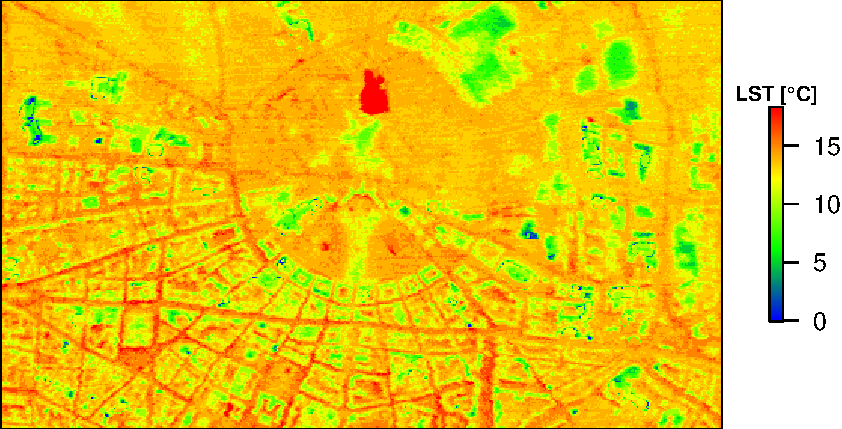
\includegraphics[width=\linewidth]{images/hotspot-rawtemp-1}
%    \label{fig:TempMaps:a}
%  \end{subfigure}
%  
%  \caption{
%    Karlsruhe city center.
%    Selected area of $2.4{\times}1.4\,km$.
%    Pixel size $5{\times}5\,m$.
%  }
%  \label{fig:TempMaps}
%\end{figure}


We define a hot spot found in comparably more coarse resolutions as
\emph{parent} (larger weight matrix or larger pixel size) and in finer
resolutions as \emph{child} (smaller weight matrix or smaller pixel size).

That is 

To be stable, one assumes that every parent has at
least one child and that each child has one parent. For a perfectly stable
interaction, it can be easily seen that the connection between parent and child
is a injective function and between child and parent a surjective function. To
measure the closeness of connection, we propose a metric called the
\emph{Stability of Hot spot} (SoH). It measures the deviation from a perfectly
stable transformation of resolutions.



In its downward property (from parent to child, injective) it is defined as:
\begin{equation}
  \label{eq:SoH-down}
  \SOHDOWN
    = \frac{ParentsWithChildNodes}{Parents}
    = \frac{|Parents \cap Children|}{|Parents|}
\end{equation}
And for its upward property (from child to parent, surjective):
\begin{equation}
  \label{eq:SoH-up}
  \SOHUP
    = \frac{ChildrenWithParent}{Children}
    = 1 - \frac{|Children - Parents|}{|Children|}
\end{equation}
where $ParentsWithChildNodes$ is the number of parents that have at least one 
\emph{child}, $Parents$ is the total number of \emph{parent}, 
$ChildrenWithParent$ is the number of children and $Children$ as the total 
number of children.
The SoH is defined for a range between 0 and 1, where 1 represents a perfectly 
stable transformation while 0 would be a transformation with no stability at 
all.

\section{Focal Getis-Ord} \label{sec:FocalGetisOrd}

\subsection{Dataset}

Our results are based on the cab taxi dataset from New York, Manhattan \cite{TODO}. 
We used only the dataset of January 2016. From that
dataset we used the $pickup\_longitude$ and $pickup\_latitude$ column. 
The borders of the raster are between (40.699607, -74.020265) and (40.769239, -73.948286). 
Zoom size 1 means we aggregate every point, which was in range of $100x100 \cdot 0.000001$ into one pixel. 
In zoom size N we aggregated NxN pixel from zoom size 1 into a new pixel.
%
For our measurements we specified the following data series:
\begin{itemize}
 \item The weight matrix W is from 3 to 43 with a stepsize of 4.
 \item The focal matrix F is from  17 to 125 with a stepsize of 12.
 \item The zoom level is from 1 to 5 with a stepsize of 1.
\end{itemize}
Therefore we calculate around $10 \cdot 10 \cdot 5=500$ results for each fixed x.
The following conditions must hold F>W, F<Raster.cols und F<Raster.rows.


\subsection{Method}

In the following text, we use the notation \FOCAL{R}{M}{op} to denote a focal
operation $op$ applied on a raster $R$ with a focal window determined by a
matrix $M$. This is rougly eqivalent to a command \verb|focal(x=R, w=M, fun=op)|
from package \emph{raster} in the R programming language \cite{cran:raster}.

\begin{definition}[$G^*$ function on rasters]
  \label{def:GenericGetisOrdFunc}
  
  The function $G^*$ can be expressed as a raster operation:
  
  \begin{displaymath}
    G^*(R, W, st) =
    \frac{
      \FOCAL{R}{W}{sum} - M*\sum_{w \in W}{w}
    }{
      S \sqrt{
        \frac{
          N*\sum_{w \in W}{w^2} - (\sum_{w \in W}{w})^2
        }{
          N - 1
        }
      }
    }
  \end{displaymath}
  \noindent where:
  \begin{itemize}
    
    \item $R$ is the input raster.
    
    \item $W$ is a weight matrix of values between 0 and 1.
    
    \item $st = (N, M, S)$ is a parametrization specific to a particular version
    of the $G^*$ function. (Def.\vref{def:StdGetisOrdVersion} and
    \vref{def:FocalGetisOrdVersion}).
    
  \end{itemize}
\end{definition}

\begin{definition}[Standard $G^*$ parametrization]
  \label{def:StdGetisOrdVersion}
  
  Computes the parametrization $st$ as global statistics for all pixels in the
  raster $R$:
  
  \begin{itemize}
    \item $N$ represents the number of all pixels in $R$.
    \item $M$ represents the global mean of $R$.
    \item $S$ represents the global standard deviation of all pixels in $R$.
  \end{itemize}
\end{definition}

\begin{definition}[Focal $G^*$ parametrization]
  \label{def:FocalGetisOrdVersion}
  
  Let $F$ be a boolean matrix such that: $all(dim(F) \geq dim(W))$.
  This version uses focal operations to compute per-pixel statistics given by 
  the focal neighbourhood $F$ as follows:
  
  \begin{itemize}
    
    \item $N$ is a raster computed as a focal operation \FOCAL{R}{F}{sum}. Each
    pixel represents the number of pixels from $R$ convoluted with the matrix
    $F$. 
    
    \item $M$ is a raster computed as a focal mean \FOCAL{R}{F}{mean}, thus each
    pixel represents a mean value of its $F$-neighbourhood.
    
    \item $S$ is a raster computed as a focal standard deviation
    \FOCAL{R}{F}{sd}, thus each pixel represents a standard deviation of its
    $F$-neighbourhood.
    
  \end{itemize}
  
\end{definition}



\section{Evaluation}

- To evaluate, we compare G* with FocalG* on the same dataset.
- We use NY taxi dropoffs
- a single evaluation run is defined in Def.~\ref{def:EvalRun}.
- In an ideal case, we could produce a 3D-plot:
  - x-axis would be growing pixel sizes 100..1000 by 100 (aka zoom-out)
  - y-axis would be growing weight matrix sizes (e.g. 5..41 by 2)
  - z-axis would be performance of G* vs FocalG* x and y coordinates
  - we could also repeat the computation for multiple datasets to obtain 
  multiple samples and to compute error bars.
- due to paper size limit, we choose projection in which matrix size is set to 
constant 7x7 pixels and the only variable is the pixel size. This way, we 
produce a 2D plot. We also generate just a single sample.

\begin{definition}[Evaluation Run]
  \label{def:EvalRun}
  We define a single evaluation run as a tuple:
  \begin{displaymath}
    E = (V, m, p, w)
  \end{displaymath}
  \noindent where:
  \begin{itemize}
  
    \item $V$ is the input dataset of points, representing the taxi dropoffs in 
    our case.
    
    \item $m$ is the metric used, in our case either \SOHUP or \SOHDOWN.
    
    \item $p$ represents the pixel size for aggregating points from $V$, 
    e.g. $100 \times 100$ meters.
    
    \item $w$ represents the size of a weight matrix.
    In our case, we chose a weight matrix depicted in 
    Figure~\ref{fig:ExampleMatrices}(a) for both the G* and FocalG* cases.
  \end{itemize}
\end{definition}

%Fig.~\ref{fig:ComparisonMorning} and Fig.~\ref{fig:ComparisonEvening} show
%Standard and Focal $G^*$ computations for both morning and eventing datasets
%with weight matrix $W$ of size 3, 5, 7, 9, 15 and 31. In this figures, when 
%computing Focal
%$G^*$, the focal matrix $F$ has a constant size of $61{\times}61$ cells. 
%Example weight matrix $W$ and focal matrix $F$ are depicted in 
%Fig.~\ref{fig:ExampleMatrices}.

\section{Methode}

The weight size W, focal size F and the zoom level are the 3 parameters we vary.
Therefore we have a 3 dimensional space. The SoH is defined for every tuple of points.
We choose to fix one dimension and used the other dimension as our sample group. 
Out of the sample group we calculate the mean and the standard deviation. 
In our graph we show the mean and the standard deviation from the mean. 
We define as a child the previous image out of the fixed dimension.


\section{Results and Discussion}

% Focal size  
%	Increase of focal size leads to better results in the upward property
% 	Standard deviation decrease with higher focal size 
%	No standard deviation af F 17x17 because of missing clusters
%	The downward property reaches its maximum at 65x65
%
%	Conclusion: F should be around 65x65 or higher

First we fixed the focal size F as our x-axis. Therefore we have no $G^*$ to compare against Focal $G^*$ because $G^*$ has a fixed study area.
To evaluate this dimension is essential because if it is not known how big the study area needs to be. Based on these results we want to fix the focal size F
so that in most cases focal $G^*$ is better than $G^*$.
In figure ~\ref{fig:SoHFocal} the \SOHUP and \SOHDOWN is shwon for $G^*$ and Focal $G^*$.
Higher values mean that the found hot spots are more stable. The \SOHUP in figure ~\ref{fig:fUp} growth with an increase of the focal size.
It can see that an increase of the focal size leads to better results for \SOHUP. 
With a higher focal size you can see that the dotted line which represent the standard deviation is getting smaller.
Therefore the standard deviation decreases with a higher focal size. Only 
at focal size F of 17x17 there is no standard deviation. Which is presented with the absent of the dotted line.
At focal size F 17x17 the standard deviation is missing, because the weight size W must be smaller than F. 
And for focal size F the values for W which are caluclated are only 3,7,11.
When F and W have similar size, there are no clusters. Because the values have no much variation. (TODO assumtion for SOH, if no clusters we asume Up/Down = 0)
\SOHDOWN can also be calculated with the same images. 
\SOHDOWN in figure ~\ref{fig:fDown} reaches its maximum for focal size F 65x65 in the regarded area. The standard deviation is not decreasing with an increase of the 
focal size. Also the standard deviation is missing for the first point. 

\begin{figure}[htp]
  \begin{subfigure}{\linewidth}
    \caption{SoH up for focal size}
    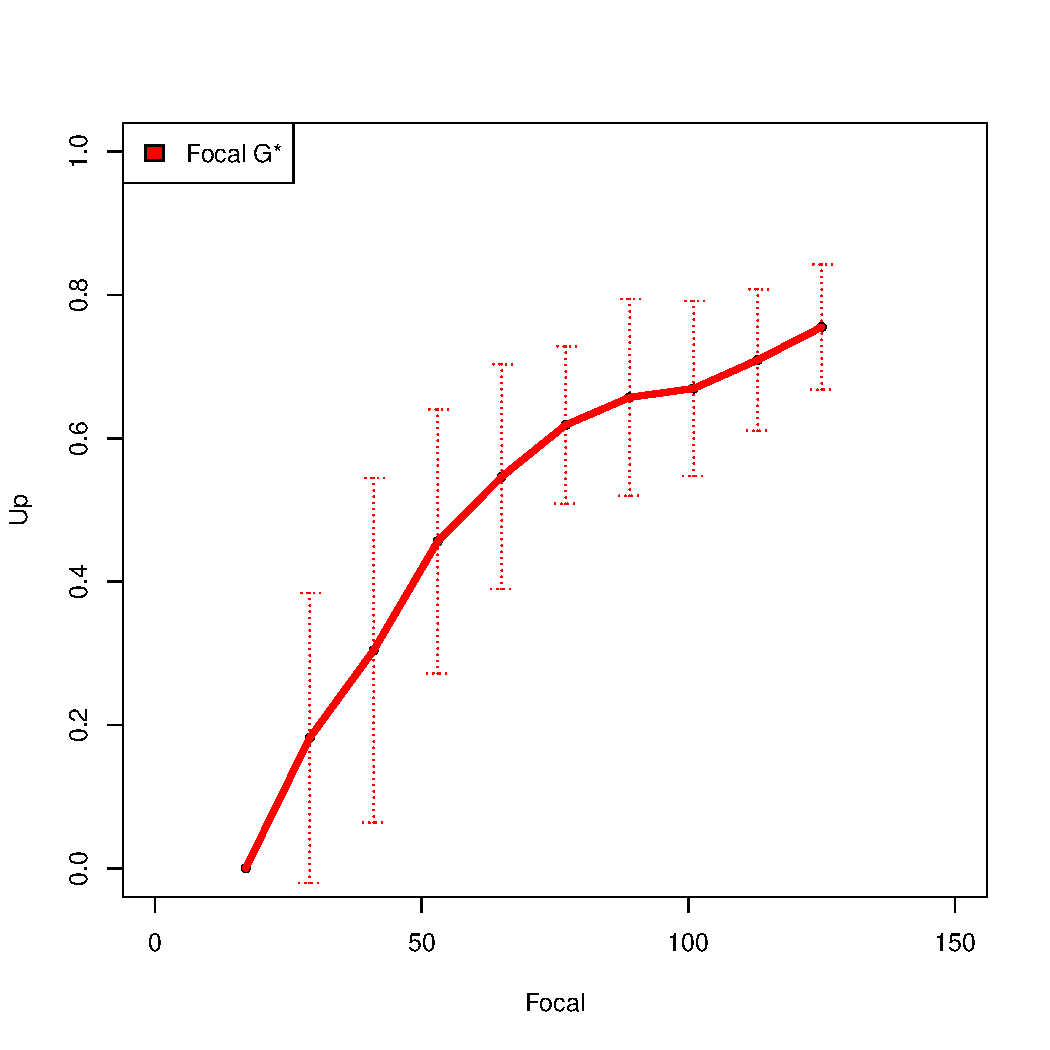
\includegraphics[width=\linewidth]{images/whiskerPlot/fUp}
    \label{fig:fUp}
  \end{subfigure}
  \hspace{1em}
  \begin{subfigure}{\linewidth}
    \caption{SoH down for focal size}
    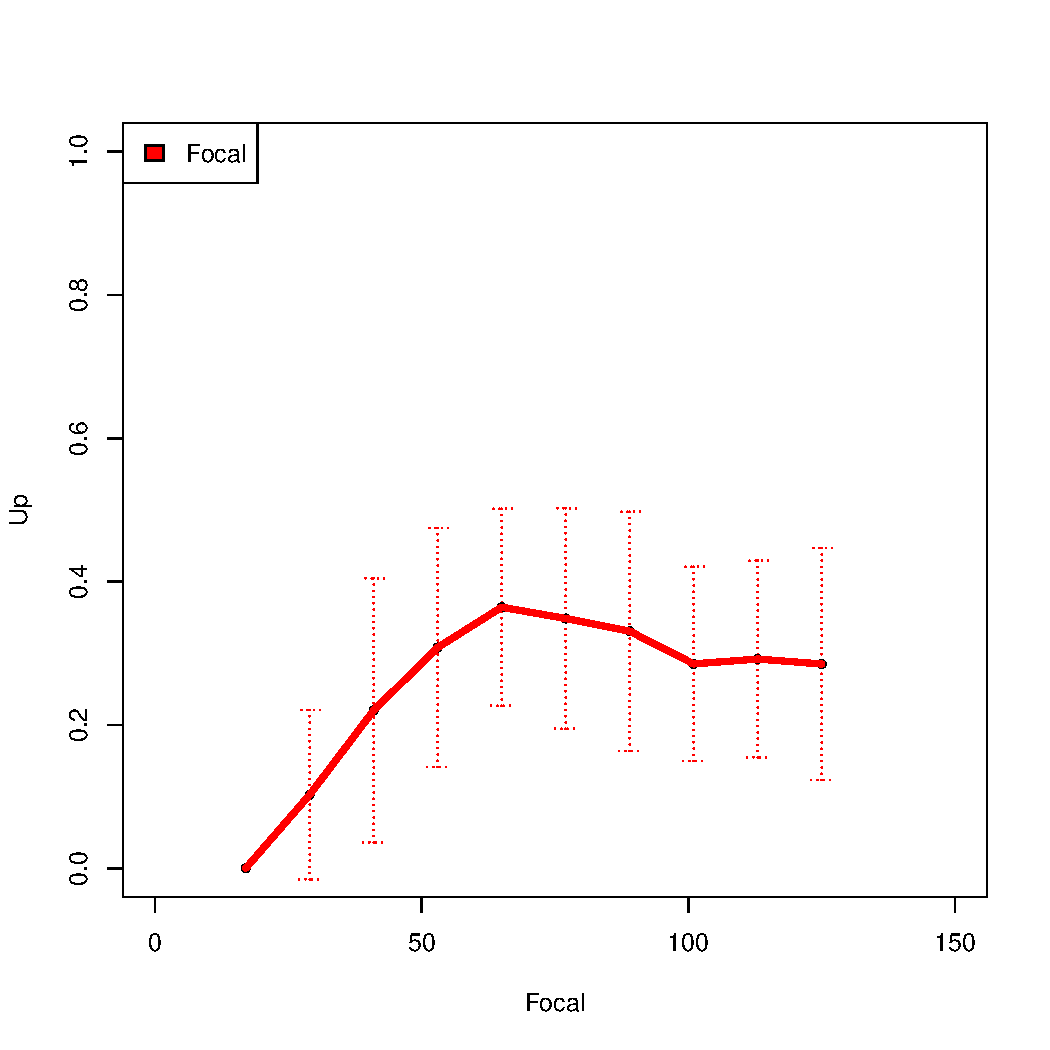
\includegraphics[width=\linewidth]{images/whiskerPlot/fDown}
    \label{fig:fDown}
  \end{subfigure}
  \caption{SoH for focal size}
  \label{fig:SoHFocal}
\end{figure}

%
% Weight size
%	Increase of weight leads to increase of downward property
%	Small break downs for G* for upward and downward property
%	For the upward property Focal G* is better than G*
%
%	Conclusion: Higher weight size leads to better results. There are parametrisations of Focal G* which are better than G*
Next we fixed the weight dimension as our x-axis. The values are increasing with an increase of the weight size W. 
Higher values means the results are more stable.
In figure ~\ref{fig:wUp} one can see that an increase of the weight size leads to better results forh the \SOHUP. 
We compare $G^*$ (blue line) wiht Focal $G^*$ (red line). The read line is not always above the blue line.
Therefore Focal $G^*$ is not allways better than $G^*$ which would be a perfect result we hoped for. It seems 
that $G^*$ has at 23 and 39 some small break downs. At first glance one would say that some parametrisation leads to that result
but the standard deviation is decreasing which indicate the opposite.
The standard deviation is in this area higher than in the other points.
In figure ~\ref{fig:wDown} the break downs are also visible which uses the same images as before but calculate the \SOHDOWN.
The high standard deviation in general indicates that it is possible to use better parametrisation for better results. Which would be the zoom size.
The break downs at 23 and 39 are also visible but this time the standard deviation is increasing.
The \SOHDOWN and \SOHUP is mostly better than $G^*$ with fixed x-axis for the weight. 
Which was the conclusion in \ref{TODO last paper}. 

\begin{figure}[htp]
  \begin{subfigure}{\linewidth}
    \caption{SoH up for weight size}
    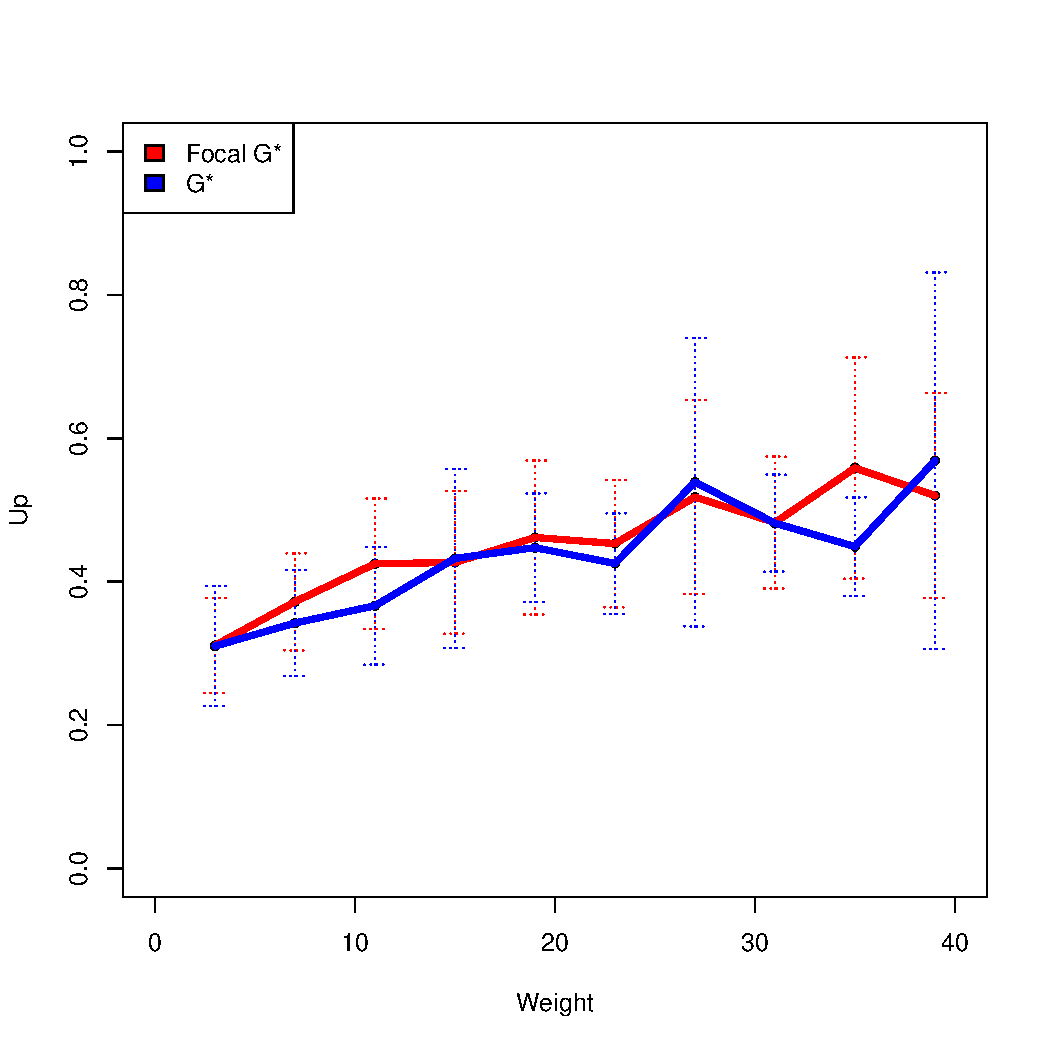
\includegraphics[width=\linewidth]{images/whiskerPlot/wUp}
    \label{fig:wUp}
  \end{subfigure}
  \hspace{1em}
  \begin{subfigure}{\linewidth}
    \caption{SoH down for weight size}
    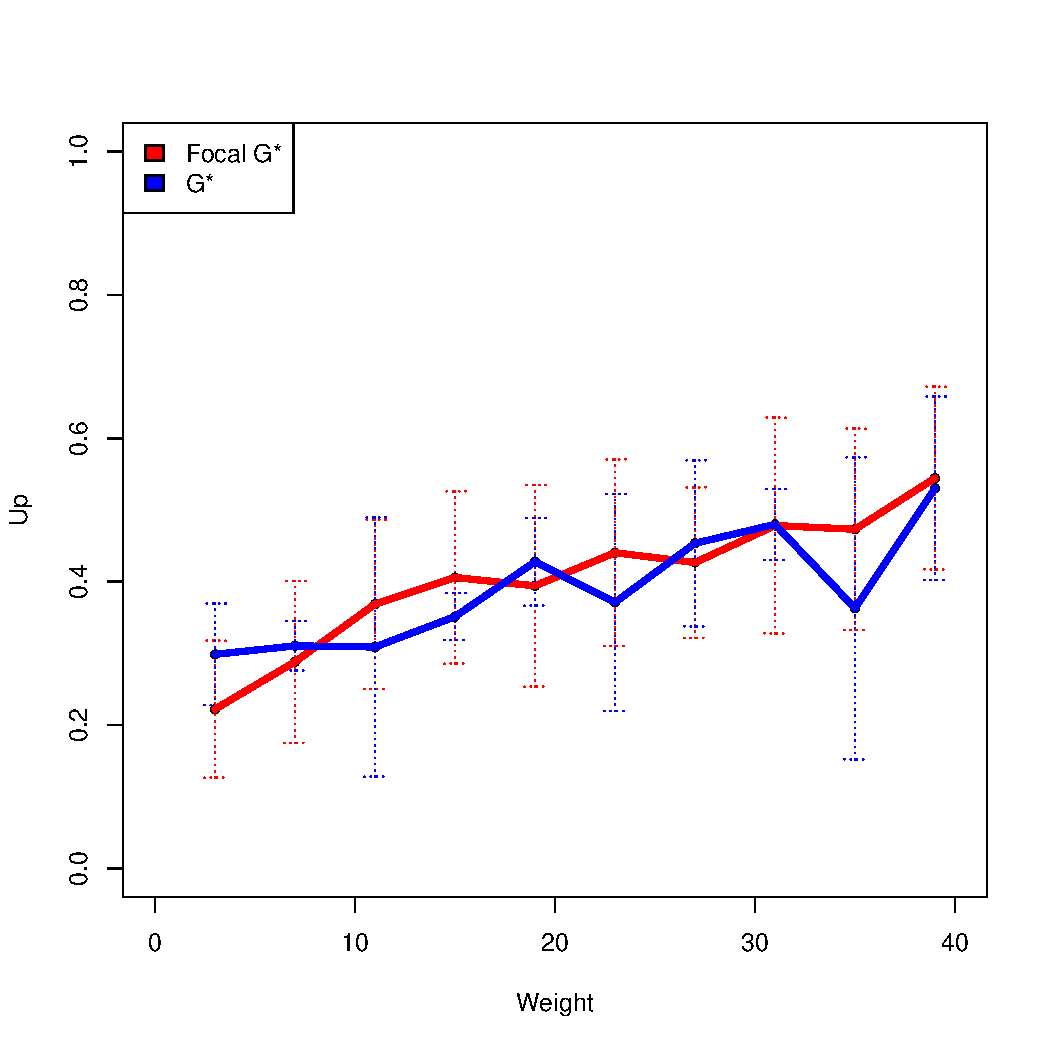
\includegraphics[width=\linewidth]{images/whiskerPlot/wDown}
    \label{fig:wDown}
  \end{subfigure}
  \caption{SoH for weight size}
  \label{fig:SoHWeight}
\end{figure}
%
% Zoom
%	G* alwas better than Focal G* for upward and downward property
%	Focal G* has different focal sizes because zoom is compared
%	At zoom level 4 G* increase much more than Focal G*
%
%	Conclusion: G* is better than Focal G* in the zoom dimension, but the focal size is fixed. The zoom dimension has the least 
%	influence on the value

The last variation we examined was the zoom level. There we fixed the x-axis as our zoom level. And the focal size and weight size variation lead to a sample set.
The results can seen in figure ~\ref{fig:SoHZoom}. For the \SOHUP there is a huge increase between zoom level 3 and 4. This increase can't be seen for \SOHDOWN.
One can see that $G^*$ is always better than Focal $G^*$. This could be beacause the target area of Focal $G^*$ increases with every zoom step. 


\begin{figure}[htp]
  \begin{subfigure}{\linewidth}
    \caption{SoH up for focal size}
    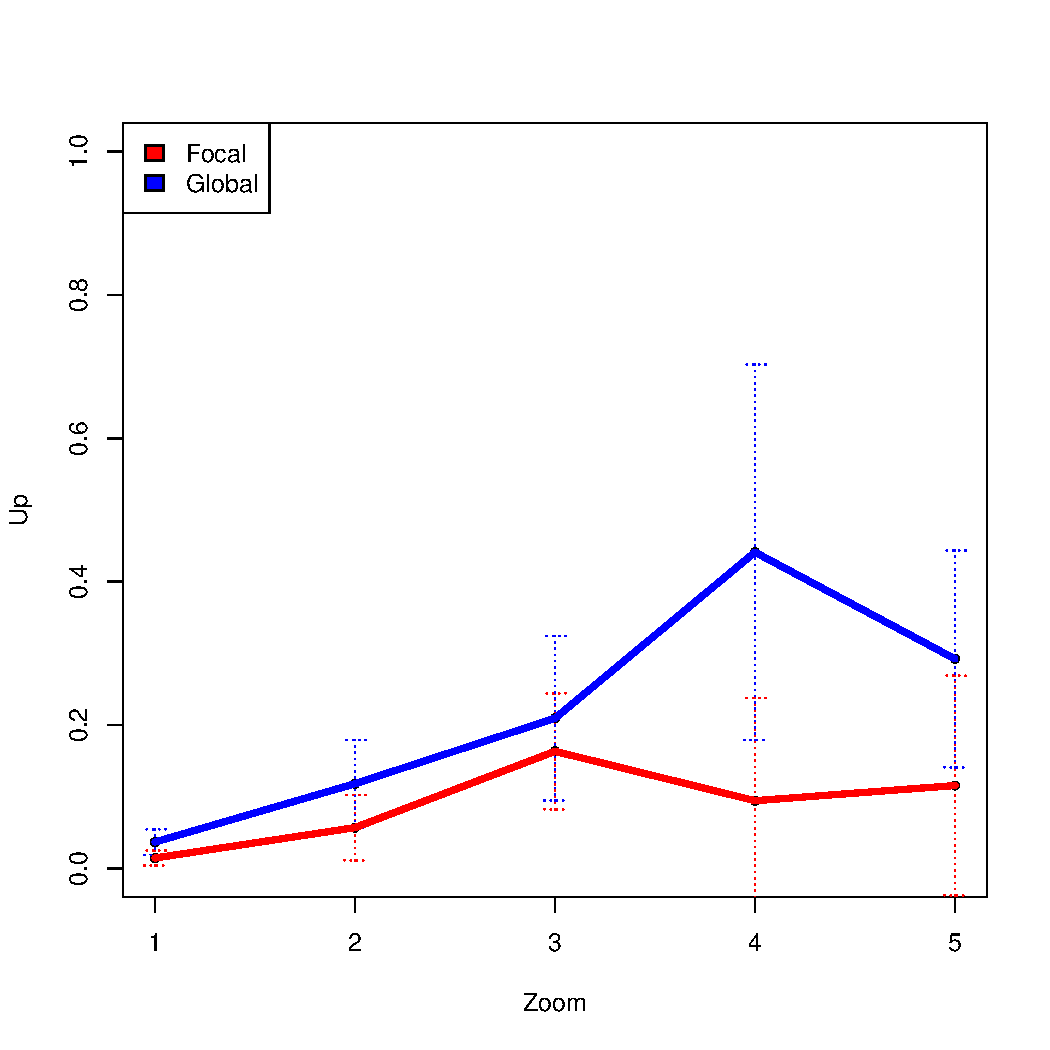
\includegraphics[width=\linewidth]{images/whiskerPlot/zUp}
    \label{fig:zUp}
  \end{subfigure}
  \hspace{1em}
  \begin{subfigure}{\linewidth}
    \caption{SoH down for focal size}
    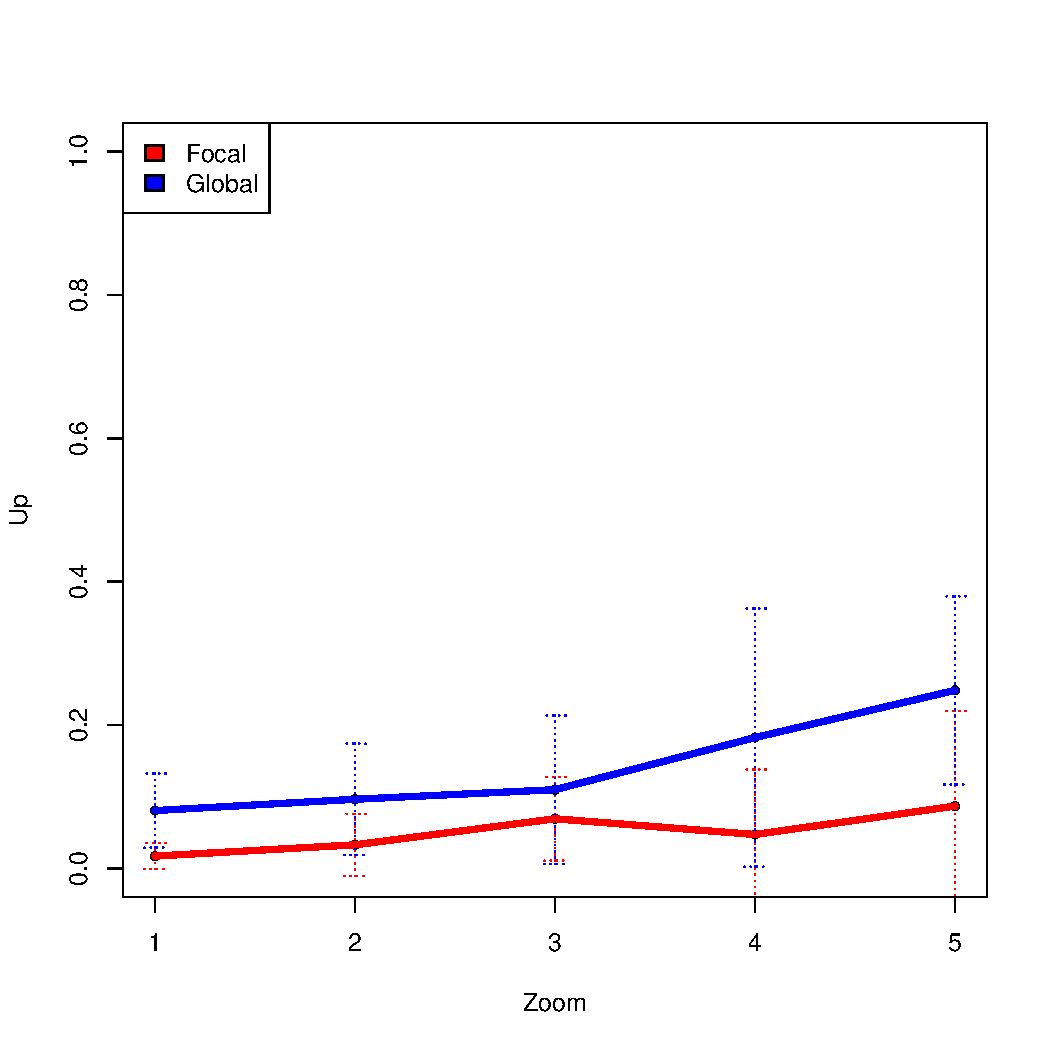
\includegraphics[width=\linewidth]{images/whiskerPlot/zDown}
    \label{fig:zDown}
  \end{subfigure}
  \caption{SoH for focal size}
  \label{fig:SoHZoom}
\end{figure}

\subsection{Clumping}

\subsection{Aggregate}

TODO settings and images
The zoom level is a slice plane through our three dimensional space. 
TODO define parent child
The results can be found in figure ~\ref{fig:Zoom}.
For the upward property, $G^*$ is always better than Focal $G^*$, compared to the results from figure
\ref{fig:SoHZoom}. Focal $G^*$ reaches the same result as $G^*$ at zoom level 5 .
For the downward property, Focal $G^*$ leads to better results at zoom level 5.

\begin{figure}[htp]
  \begin{subfigure}{\linewidth}
    \caption{Upward for zoom}
    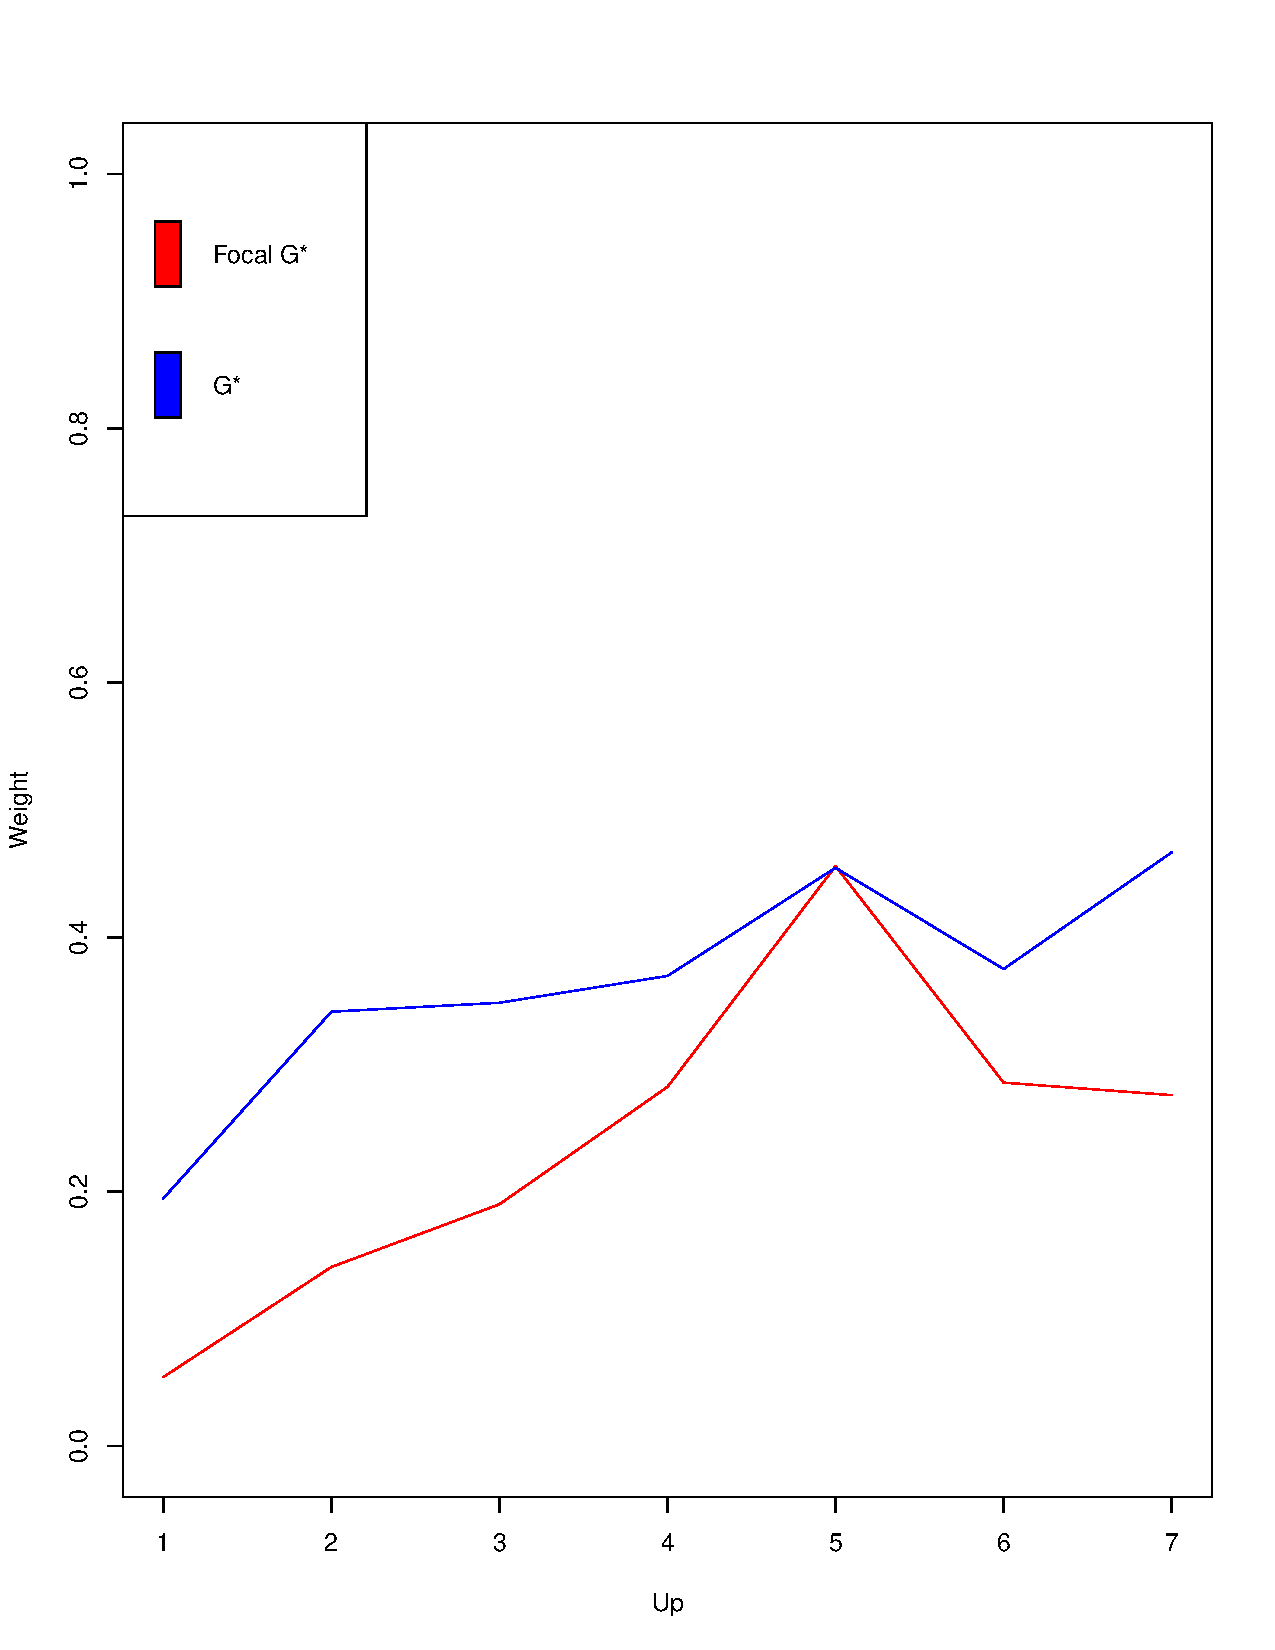
\includegraphics[width=\linewidth]{images/SoHZoomUp}
    \label{fig:UpwardZoom}
  \end{subfigure}
  \hspace{1em}
  \begin{subfigure}{\linewidth}
    \caption{Downward for zoom}
    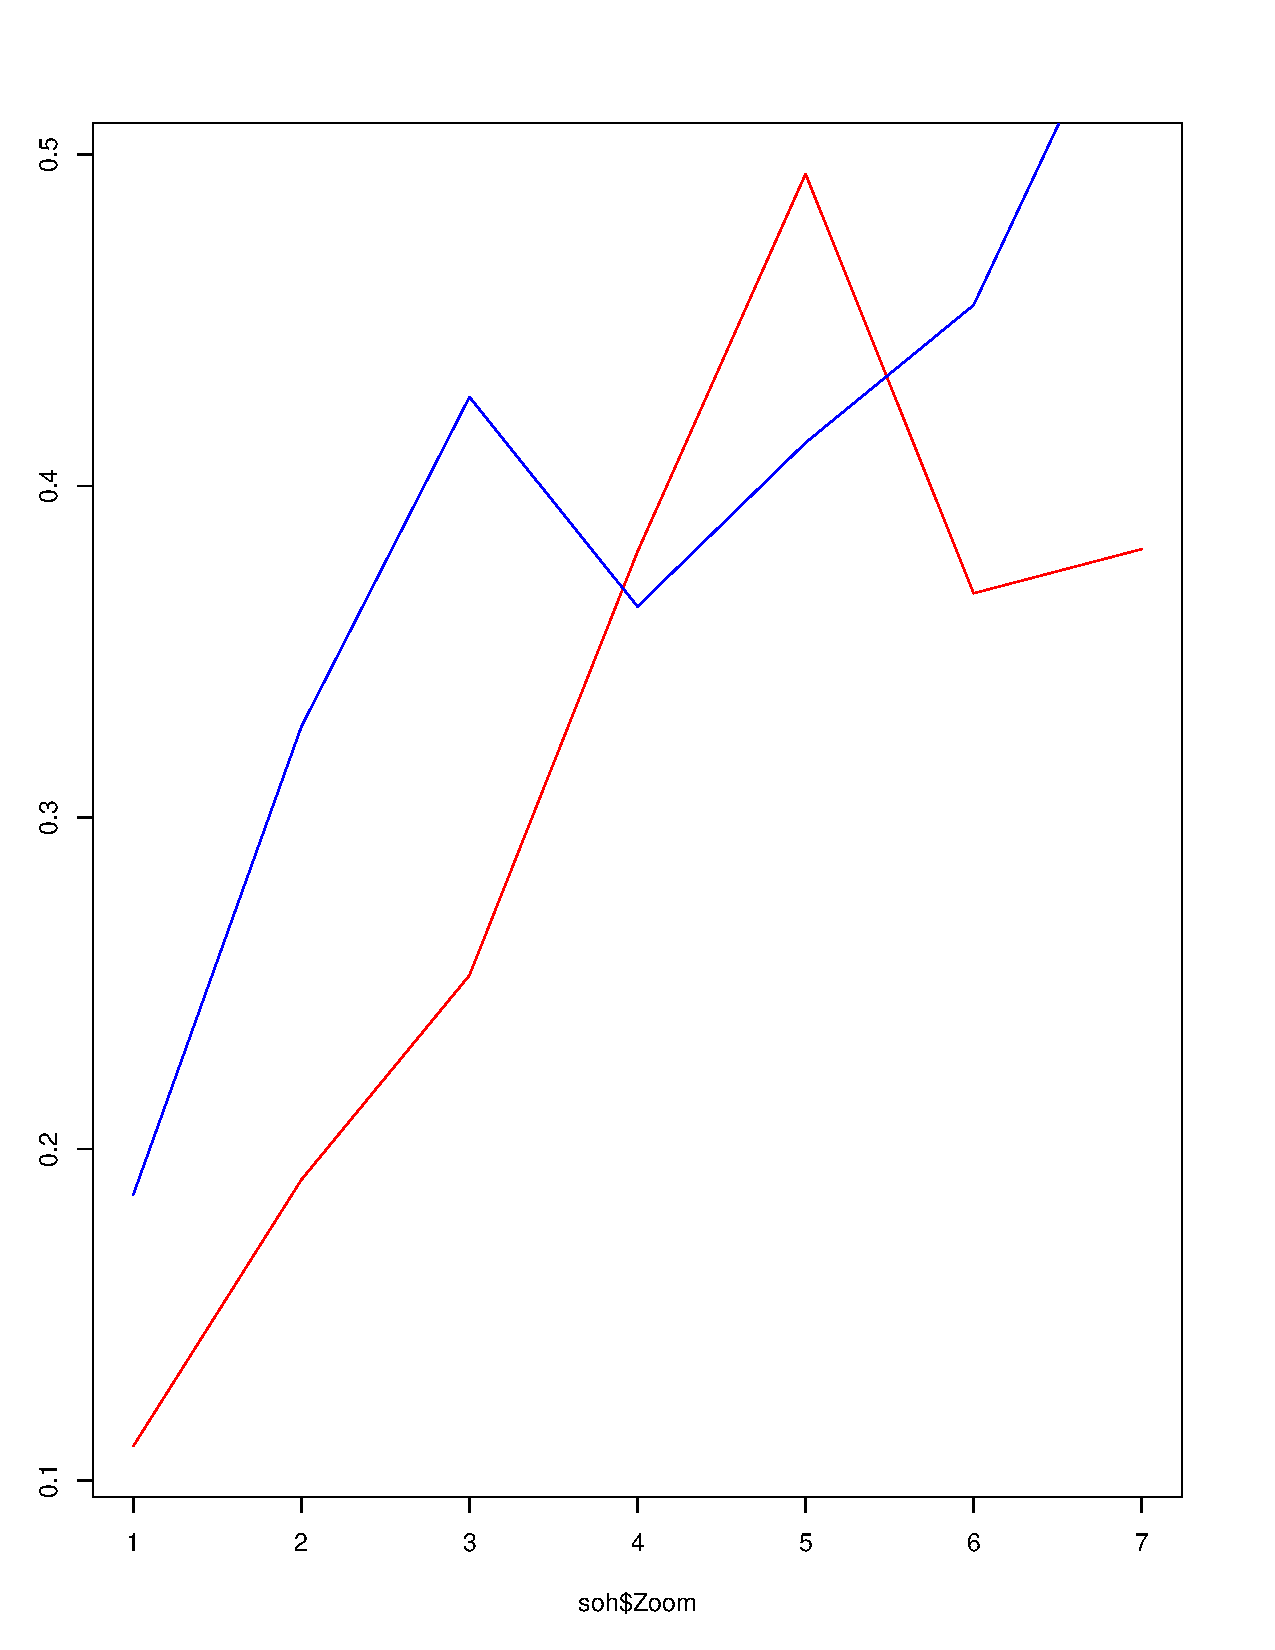
\includegraphics[width=\linewidth]{images/SoHZoomDown}
    \label{fig:DownwardZoom}
  \end{subfigure}
  \caption{SoH zoom}
  \label{fig:Zoom}
\end{figure}


\subsection{Blur}

The evaluation results are plotted in Fig.~\ref{fig:Blur}, each point in
the graph represents the \SOHUP metric (Eq.\ref{eq:SoH-up}) between two
$G^*$ generated using weight matrices of size $i$ and $i+2$. The focal matrix F
has a fixed size of $41{\times}41$

\begin{displaymath}
\SOHUP( G^*(R, W_i, st), G^*(R, W_{i+2}, st) )
\end{displaymath}


The slice plane of the weight dimension is consistent with figure ~\ref{fig:SoHWeight}.
Higher weight leads in general to better results for Focal $G^*$. $G^*$ doesn't fit to the mean of our whiskerplot.


\begin{figure}[htp]
  \begin{subfigure}{\linewidth}
    \caption{Upward for blur}
    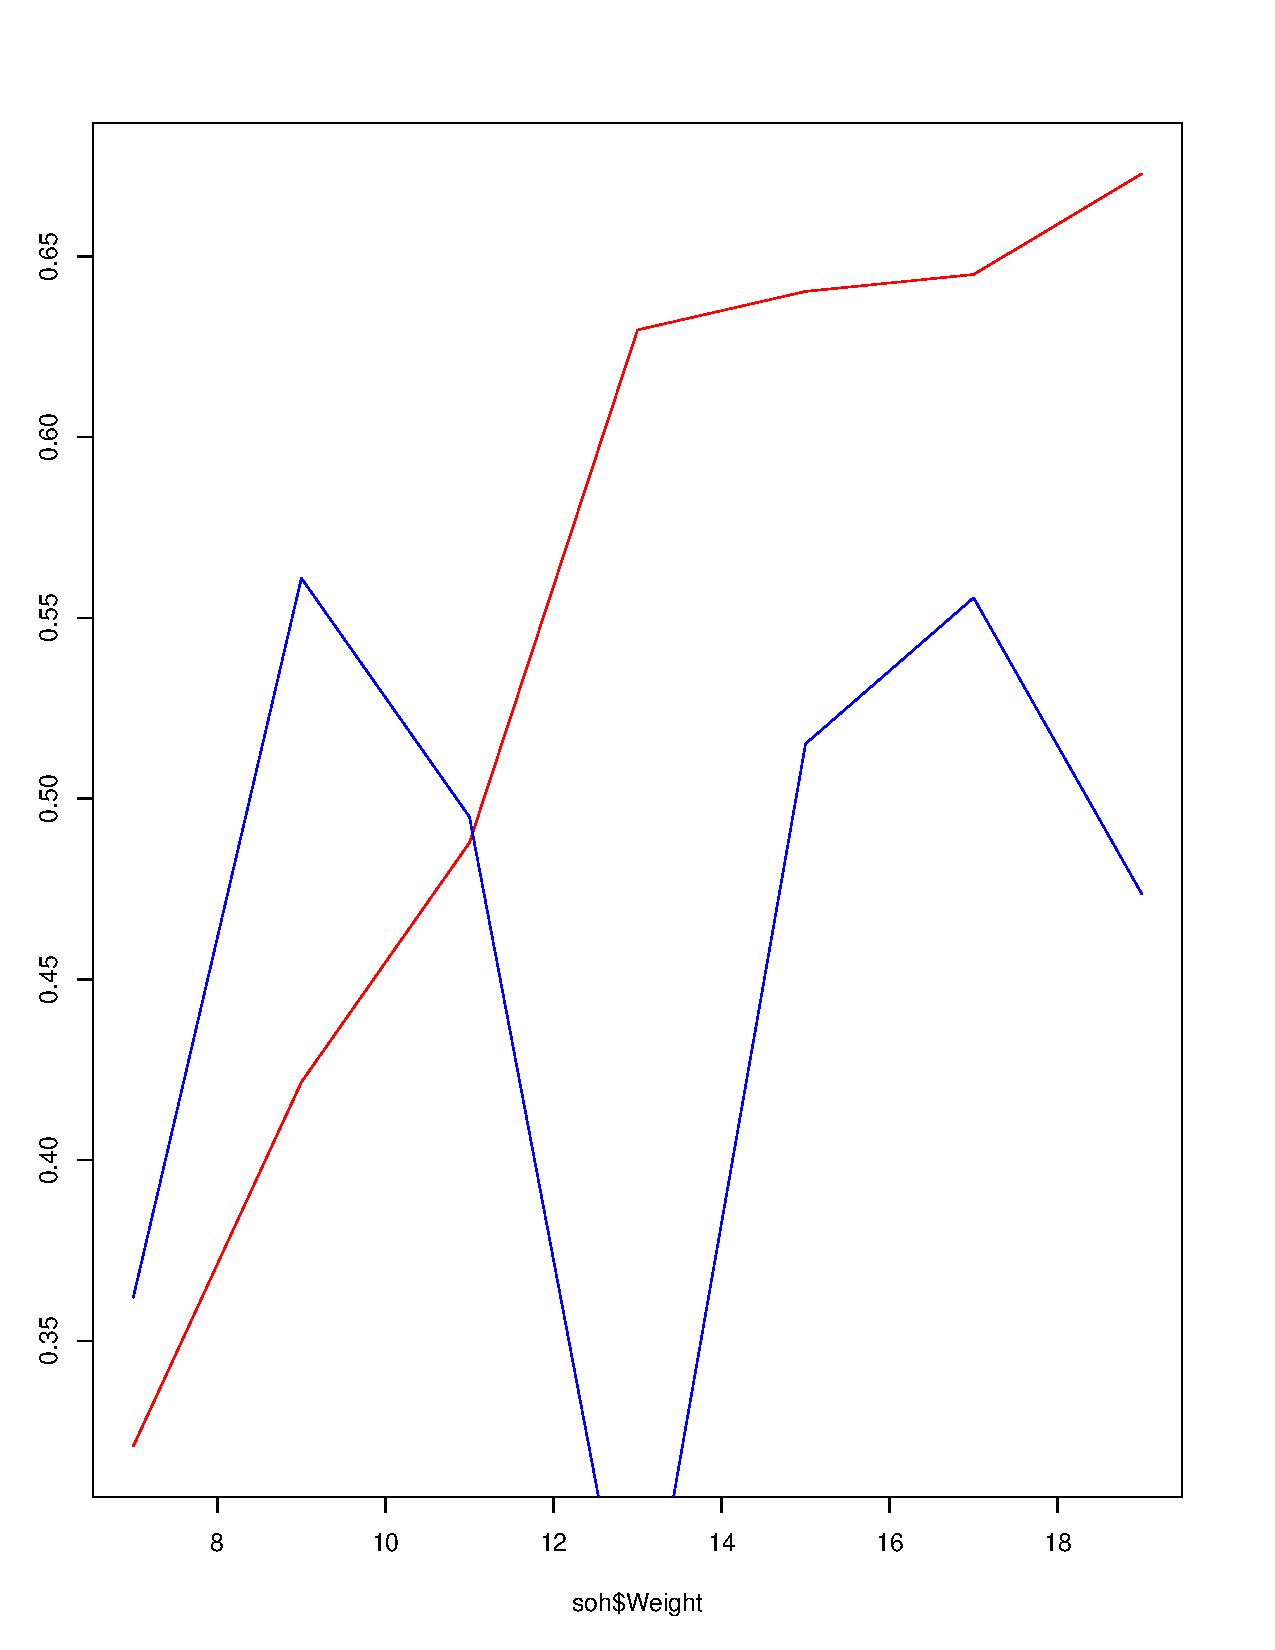
\includegraphics[width=\linewidth]{images/SoHUpBlur}
    \label{fig:UpwardBlur}
  \end{subfigure}
  \hspace{1em}
  \begin{subfigure}{\linewidth}
    \caption{Downward for blur}
    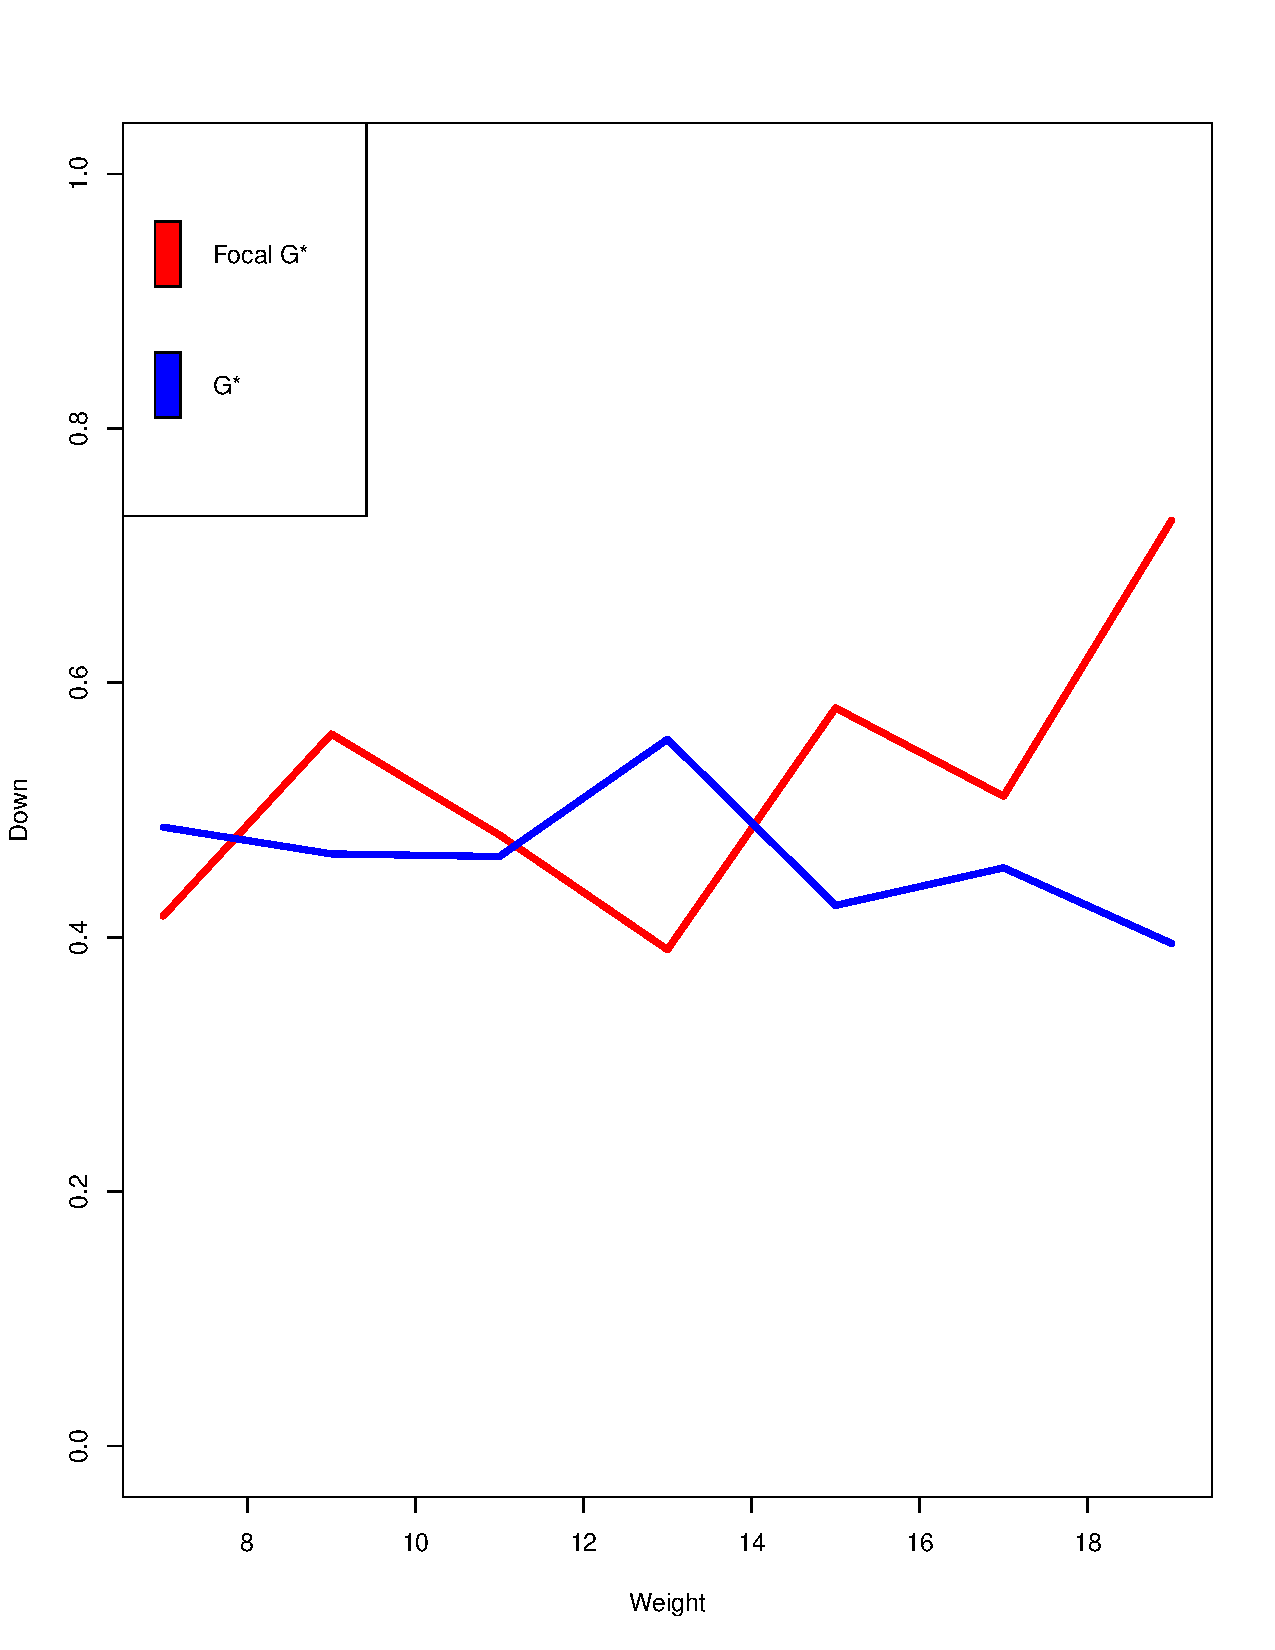
\includegraphics[width=\linewidth]{images/SoHDownBlur}
    \label{fig:DownwardBlur}
  \end{subfigure}
  \caption{SoH blur}
  \label{fig:Blur}
\end{figure}


\section{Conclusions and Future Work} \label{sec:Conclusion}
In this work, we compared the Getis-Ord statistic with Focal Getis-Ord statisitic. We validate the result from \ref{TODO last paper} with a real world 
dataset an with a larger dataset. The dataset was only one month projected in one raster. 
We examined further parameters and evaluated that $G^*$ and Focal $G^*$ performe better if the weight
is higher.
Our results indicate a high Focal range for the upward property and a maximum of 65x65 for the downward property.
Therefore F should be not less than 65x65. 
If we calculate the SoH for the zoom level, Getis-Ord leads to better results. In general the zoom level 
has the least influence if $G^*$ or Focal $G^*$ performe better.
We assume that if Focal $G^*$ has a different focal size for a different zoom level, 
it performes better, but this is beyond the scope of this work.

With this work we made a step further to the optimal parametrisation for $G^*$ and Focal $G^*$.
Our results indicate that the parametrisation for $G^*$ and Focal $G^*$ besides what is defined as parent and child has a huge impact on the
stability of hotspots. Wrong parametrisation can lead to good results, the mean reaches for \SOHUP in the weight dimension around 0.6.
It can also lead to bad result, \SOHUP in the zoom dimension reaches nearly zero. Therefore we shown that it is important to have a metric
for the stability of hotspots. Also we presented indication which parametrisation should be avoided and which parametrisations are promising.
$G^*$ can also be applied to spatio-temporal data.
Therefore Focal $G^*$ should be also applied to the spatio-temporal data. 
We now have a good indication which weight and focal size is usefull.
We didn't evaluate the results on other month because we assume that they are similar But it is interesting to find clusters for different times in the day.
One could asume that at lunchtime there will be hotspots at restaurants and they are not consistent with the hotspots over one month.
All our results are based on the SoH. Further work should validate or improve this metric also for the temporal dimension.





\section{Acknowledgements}
This work is part of the research project BigGIS (reference number: 01IS14012)
funded by the Federal Ministry of Education and Research (BMBF) within the
frame of the programme "Management and Analysis of Big Data" in "ICT 2020 --
Research for Innovations".
We thank the Nachbarschaftsverband Karlsruhe for the data of the thermal flight
over Karlsruhe. %
\noindent R-packages used: \verb|raster|~\cite{cran:raster}, 
\verb|knitr|~\cite{cran:knitr}

\bibliographystyle{plain}
\bibliography{bibfile}  % sigproc.bib is the name of the

\end{document}
